\chapter{Методология измерения ЭДМ и её систематические ошибки}

\section{Общее введение в методологию ``Замороженного Спина'' (FS)}
\subsection{Уравнение Т-БМТ}\label{sec:TBMT_introduction}
Уравнение Томаса-БМТ описывает динамику спин-вектора $\vec s$ в
магнитном поле $\vec B$ и электростатическом поле $\vec E$. Его
обобщённая версия, включающая влияние ЭДМ, может быть записана (в
системе центра масс пучка) как:~\cite[стр.~6]{Eremey:Thesis}
\begin{subequations}
  \begin{align}
    \ddt{\vec s} &= \vec s\times \bkt{\vec\W_{MDM} +\vec\W_{EDM}}, \label{eq:TBMT_main}
    \intertext{где МДМ и ЭДМ угловые скорости $\vec\W_{MDM}$ и $\vec\W_{EDM}$ }
    \vec\W_{MDM} &= \frac qm \bkt*{G\vec B - \bkt{G - \frac{1}{\gamma^2-1}}\frac{\vec E\times\vec\beta}{c}},\label{eq:TBMT_MDM} \\
    \vec\W_{EDM} &= \frac qm \frac\eta2 \bkt*{\frac{\vec E}c + \vec\beta\times \vec B}.\label{eq:TBMT_EDM}
  \end{align}
\end{subequations}
В уравнениях выше, $m,~q,~G=(g-2)/2$ есть, соответственно, масса, заряд, и
магнитная аномалия частицы; $\beta = \sfrac{v_0}{c}$,
нормализованная скорость частицы; $\gamma$ её Лоренц-фактор. ЭДМ
множитель $\eta$ определяется уравнением $d = \eta\frac{q}{2mc}s$, где
$d$ --- ЭДМ частицы, а $s$ её спин.

В стандартном формализме принято оперировать с матрицей преобразования (поворота) спина за оборот в кольце $R$:~\cite[стр.~4]{COSY:SpinTuneMapping}
\[
\bold{t}_R = \exp\bkt{-i\pi\nu_s\vec\sigma\cdot\bar n} = \cos\pi\nu_s - i (\vec\sigma\cdot\bar n)\sin\pi\nu_s,
\]

где $\nu_s = \sfrac{\W_s}{\W_{cyc}}$ отношение угловой скорости поворота спин-вектора частицы к её циклотронной частоте, называемое \emph{спин-тюн}, а $\bar n$ определяет направление оси прецессии спина, и называется \emph{инвариантной спиновой осью}.

\subsection{Концепция замороженного спина}
Из уравнения~\eqref{eq:TBMT_MDM} можно видеть, что, в отсутствии ЭДМ,
направление вектора спина частицы пучка может быть зафиксировано
относительно её вектора импульса: $\vec\W_{MDM}=\vec 0$; иными словами, можно реализовать
условие замороженности спина (Frozen Spin condition).

Достоинством налагания FS-условия на пучок в накопительном кольце
следующее: в соответствии с
уравнениями~\cref{eq:TBMT_main,eq:TBMT_MDM,eq:TBMT_EDM}, векторы МДМ и
ЭДМ угловых скоростей ортогональны, а потому в общей скорости
прецессии они складываются квадратично, в связи с чем сдвиг частоты
прецессии, связанный с ЭДМ, становится эффектом второго порядка
величины:~\cite[стр.~5]{Mane:SpinWheel}
\[
\w \propto \sqrt{\W_{MDM}^2 + \W_{EDM}^2} \approx \W_{MDM} + \frac{\W_{EDM}^2}{2\W_{MDM}}.
\]
Это обстоятельство значительно ухудшает чувствительность эксперимента.

Однако, заморозив спин в горизонтальной плоскости, единственная
осающаяся МДМ компонента угловой скорости сонаправлена с ЭДМ
компонентой, а значит складывается с ней линейно. Таким образом,
чувствительность значительно улучшается.

\subsection{Реализация условия замороженности спина в накопительном кольце}\label{sec:FS_in_a_ring}
Накопительные кольца могут быть классифицированы в три группы:
\begin{enumerate}
\item чисто магнитные (как COSY, NICA, etc),
\item чисто электростатические (Brookhaven AGS Analog Ring),
\item комбинированные.
\end{enumerate}

Ввиду уравнения~\eqref{eq:TBMT_MDM}, условие FS не может быть
выполнено в чисто магнитном кольце.

Для некоторого числа частиц, таких как протон, чья $G>0$, чисто
электростатическое кольцо может быть использовано в рамках FS
методологии ЭДМ эксперимента с пучком на так называемой ``магической''
энергии, определяемой как $\gamma_{mag} = \sqrt{(1+G)/G}$.

Для частиц с $G<0$ (таких как дейтрон),это невозможно, и необходимо
использовать комбинированное кольцо. Для того, чтобы реализовать FS
условие в комбинированном кольце, вводится ~\cite{BNL:Deuteron2008} радиальное электрическое
поле величины
\begin{equation}\label{eq:FS_Er}
  E_r = \frac{GB_yc\beta\gamma^2}{1-G\beta^2\gamma^2}.
\end{equation}

\section{Методы, основанные на FS-методологии} \label{sect1_2}
\subsection{Метод BNL FS}
BNL FS метод, предложенный коллаборацией, занимающейся разработкой
метода измерения ЭДМ в накопительном кольце в Брукхейвенской
Национальной Лаборатории (США) в 2008 году,~\cite{BNL:Deuteron2008}
это метод для комбинированного кольца. Пучок продольно-поляризованных
дейтронов инжектируется в кольцо; с помощью поляриметрии наблюдается
его спин-прецессияв вертикальной и горизонтальной плоскостях; ЭДМ
сигнал --- это изменение вертикальной компоненты поляризации со
временем, выражаемое как:~\cite[стр.~8]{BNL:Deuteron2008}
\begin{equation}
  \Delta P_V = P\frac{\w_{edm}}{\W}\sin\bkt{\W t + \Theta_0},
\end{equation}
где $\W = \sqrt{\w_{edm}^2 + \w_a^2}$, $\w_a,~\w_{edm}$ угловые
скорости вызываемые, соответственно, магнитным и электрическим
дипольными моментами.

Налагая радиальное магнитное поле $E_r$~\eqref{eq:FS_Er}, ожидается
уменьшение компоненты $\w_a$ по крайней мере на фактор $10^9$; ввиду
малости величины гипотезируемой $\w_{edm}$, $\Delta P_V \approx P
\w_{edm} t$, и максимальная величина $\Delta P_V$ возрастает в $10^9$.

Ожидаемая чувствительность эксперимента $10^{-29}~e\cdot cm$ за $10^7$
секунд (6 месяцев) полного времени измерения. На этом уровне
чувствительности, асимметрия сечения $\varepsilon_{LR} \approx 5\cdot
10^{-6}$ для наименьших практически реализуемых значений
$\w_a$.~\cite[стр.~18]{BNL:Deuteron2008} Последнее обстоятельство
ставит серьёзную проблему для поляриметрии.~\cite{Mane:SpinWheel} Один
из вариантов её решения лежит в применении внешнего радиального
магнитного поля и измерении обзей частоты прецессии засчёт МДМ и ЭДМ
вместе. Это основа так называемого метода Spin Wheel, о котором в
следующем разделе.

Единственный известный систематический эффект спиновой динамики
первого порядка это присутствие ненулевой средней вертикальной
компоненты электрического поля $\avg{E_V}$. В этом случае, спин будет
прецессировать вокруг радиального направления с частотой~\cite[стр.~11]{BNL:Deuteron2008}
\[
\w_{syst} \approx \frac{\mu\avg{E_V}}{\beta c\gamma^2}.
\]
Здесь важно рассмотреть два обстоятельства:
\begin{itemize}
\item присутствие $\avg{E_V}\neq 0$ вызвано ошибкой юстировки
  элементов ускорителя;
\item этот систематический эффект меняет знак при инжекции пучка в
  обратном направлении.
\end{itemize}
Последнее обстоятельство является причиной структуры инжекции пучка
использованной в этом методе (сначала по-часовой, потом
против-часовой; CW/CCW). Хотя $\w_{syst}$ меняет знак при смене
направления движения пучка, эта методология тем не менее не учитывает
его \emph{величину}. В разделах~\ref{sec:systematic_error-fake_signal} и~\ref{sec:simulation-fake_signal}, 
мы
показываем, что при реалистичной величине ошибки установки
спин-ротаторов 100 мкм, частота МДМ прецессии вокруг радиальной оси
находится на уровне 50--100 рад/сек.~\cite{Senichev:FDM} В связи с
этим, невозможно использовать данную методологию в её оригинальном варианте.

\subsection{Spin Wheel концепция}
Озвученные выше проблемы с поляриметрией и высокой скоростью прецессии
решаются в Spin Wheel (SW) модификации, предложенной проф. И. Коопом
(Новосибирский Государственный Университет). Основная идея метода в
следующем: сначала, обеспечивается условие замороженного спина; затем
включается радиальное магнитное поле величины $B_x$, достаточно сильное чтобы
вызвать вращение спина с частотой порядка 1 Гц. Поскольку поле
радиальное, вызванная им МДМ прецессия сонаправлена с ЭДМ, а значит
они складываются линейно: $\w \propto \W_{MDM} + \W_{EDM}$.

ЭДМ вклад вычисляется сравнением циклов с обратными знаками $B_x$:~\cite[стр.~1963]{Koop:IPAC13}
\[
\W_{EDM} = \frac{\W_x(+B_x) + \W_x(-B_x)}{2}.
\]

Внешнее поле также вызовет разделение орбит
пучков.~\cite[стр.~1963]{Koop:IPAC13} Это разделение может быть
измерено на уровне пико-метров SQUID магнетометрами; его предлагается
использовать для калибровки внешнего поля.

Поскольку из-за внешнего поля прецессия вокруг радиальной оси на 10
порядков выше чем в оригинальном предложении, значительно упрощается
задача для поляриметрии. Однако, существуют сомнения в возможности
измерить вызываемое внешним полем разделение орбит даже при помощи SQUIDов.

Также, проблема паразитного поля, вызванного ошибкой юстировки, не решена.

\subsection{Метод Frequency Domain}\label{sec:FDM_concept}
Методология Frequency Domain (далее FDM)~\cite{Senichev:FDM} была разработана специально для решения проблемы неточности установки магнитов, и возникающего в связи с этим паразитного МДМ вращения спина. Как было обозначено выше, частота вращения спина в вертикальной плоскости, связанная с магнитным дипольным моментом, при реалистичной ошибке юстировки, находится на уровне 8--16 Гц, что делает невозможным наблюдение медленного нарастания вертикальной компоненты поляризации, связанное с наличием у частицы электрического дипольного момента, как предполагается оригинальным BNL FS методом. В FDM, ЭДМ-эффект вычисляется путём сравнения комбинированной (МДМ + ЭДМ) частоты прецессии, наблюдаемой при циркуляции пучка в прямом и обратном направлениях. Поскольку при смене полярности ведущего поля $\vec B \mapsto -\vec B$, $\vec\beta \mapsto -\vec\beta$, и $\vec E \mapsto \vec E$:
\begin{subequations}
  \begin{align}
    \w_x^{CW/CCW} &= \w_x^{MDM, CW/CCW} + \w_x^{EDM, CW/CCW}, \\
    \w_x^{MDM, CW} &= -\w_x^{MDM, CCW} \equiv \w_x^{MDM}, \label{eq:FDM_CW_CCW_MDM} \\
    \w_x^{EDM, CW} &= \w_x^{EDM, CCW} \equiv \w_x^{EDM},
    \intertext{поэтому, ЭДМ эстиматор}
    \hat\w_x^{EDM} &:= \frac12\bkt{\w_x^{CW} + \w_x^{CCW}} \label{eq:FDM_estimator} \\
                  &= \w_x^{EDM} + \underbrace{\frac12\bkt{\w_x^{MDM, CW} + \w_x^{MDM, CCW}}}_{\varepsilon \to 0}.
  \end{align}
\end{subequations}

Для того, чтобы гарантировать малость $\varepsilon$ по сравнению с требуемой точностью измерений, т.е., что уравнение~\eqref{eq:FDM_CW_CCW_MDM} выполняется достаточно точно, была разработана специальная процедура смены полярности ведущего поля, описанная в разделе~\ref{sec:field_flipping-theory}.

\subsubsection{Смена полярности ведущего поля}\label{sec:field_flipping-theory}
Как было описано в разделе~\ref{sec:FDM_concept}, для того, чтобы исключить МДМ-эффект из конечной статистики эксперимента, построенного на основе Frequency Domain методологии в комбинированном накопительном кольце, необходимо произвести смену полярности ведущего магнитного поля. Электростатическое поле $E_r = \frac{GB_yc\beta\gamma^2}{1-G\beta^2\gamma^2}$ (см. раздел~\ref{sec:FS_in_a_ring}) при этом фиксировано.

Частоты прецессии спинов частиц пучка определяются по формуле~\cite[стр.~4]{COSY:SpinTuneMapping}
\[
(\W_x, \W_y, \W_z) = 2\pi\cdot f_{rev} \cdot \nu_s \cdot \bar n,
\]
где $f_{rev}$ есть циклотронная частота частицы, а $\nu_s$ и $\bar n$ --- её спин-тюн и ось стабильного спина, соответственно. В разделе~\ref{sec:decoherence_simulations} мы приведём свидетельства того, что при использовании секступольных полей выравниваются не только спин-тюны частиц, но и направления их осей стабильного спина, в связи с чем в дальнейшем рассмотрении мы будем предполагать что спин-векторы всех частиц в пучке вращаются вокруг $\bar n^{CO}$, определённой на референсной орбите. Таким образом, при смене полярности ведущего поля достаточно восстановить эффективный Лоренц-фактор пучка, для того, чтобы восстановить величину угловой скорости паразитной МДМ прецессии.

Калибровка $\gamma_{eff}$ выполняется напрямую, через восстановление угловой скорости прецессии спина в горизонтальной плоскости:
В начальном состоянии, $\W_x\gg \W_y, \W_z$, и $\bar n^{CO}\approx \hat x$. Используя спин-суппрессор (Вин-фильтр), мы подавляем прецессию вокруг вектора $\hat x$; одновременно с этим, мы отходим от ``замороженного'' значения энергии (это делается для того, чтобы избежать неустойчивого состояния ``заморозки'' спина во всех плоскостях). При изменении энергии пучка, меняется также и величина ведущего поля, за тем, чтобы сохранить референсную орбиту. Горизонтальная прецессия становится доминантной, и $\bar n^{CO} \approx \hat y$. После смены полярности ведущего поля, мы опять подстраиваем его величину таким образом, чтобы восстановить условие замороженности спина в горизонтальной плоскости. Тогда, при выключении спин-суппрессора, и возвращении энергии пучка на изначальный уровень, мы получаем $\bar n^{CO} \approx -\hat x$, $\gamma_{eff}^{CCW} = \gamma_{eff}^{CW}$, то есть, МДМ прецессия происходит с той же угловой скоростью, но в обратном направлении. 

Также отметим, что существуют методы измерения ЭДМ элементарных частиц, не основанные на принципе замороженного спина; например~\cite{COSY:SpinTuneMapping}

\section{Анализ систематических ошибок} \label{sec:systematic_error}
\subsection{Возмущение оси прецессии спина частицы засчёт бетатронного движения}
\subsubsection{Мотивация изучения эффекта}
Инвариантная спиновая ось частицы, учавствующей в бетатронном движении, колеблется вокруг своего референсного значения.~\cite[стр.~11]{Shatunov} По этой причине, \hl{амплитуда решения уравнения}\footnote{Здесь бы не помешала ссылка.} Т-БМТ для вертикальной компоненты спин-вектора:
\begin{align}
s_y &= \sqrt{\bkt{\frac{\w_y\w_z}{\w}}^2 + \bkt{\frac{\w_x}{\w}}^2}\cdot\sin\bkt{\w\cdot t + \phi}\notag\\
&= \sqrt{\bkt{\bar n_y\bar n_z}^2 + \bar n_x^2} \cdot \sin\bkt{2\pi\cdot\nu_s\cdot n_{turn} + \phi},\label{eq:sy_varying_amplitude}
\end{align}
превращается в изменяющуюся во времени функцию. В связи с этим, использование простой гармонической функции в качестве модели для фитирования сигнала влечёт за собой систематическую ошибку спецификации модели. Ошибки данного типа отражаются на валидности оценок параметров модели, то есть на оценке частоты, и потому требуют анализа.

\subsubsection{Значимость эффекта}
Мы изучили данный эффект, и пришли к выводу, что он пренебрежимо мал. На Рисунке~\ref{fig:n-bar_optimized} изображены компоненты оси прецессии спина, вычисленные на фазовых траекториях частиц (Рисунок~\ref{fig:phase_space}), в структуре, использующей секступольные поля для подавления декогеренции в вертикальной плоскости. Для наглядности, все компоненты $(\bar n, \nu_s)$, построенные друг против друга, представлены на Рисунке~\ref{fig:all_vs_all}. Как можно наблюдать из Рисунков, продольная компонента имеет максимальную амплитуду колебаний на уровне $10^{-5}$, в то время как $\bar n_x$, $\bar n_y$ колеблются вокруг своих средних значений с амплитудами, соответственно, $10^{-9}$ и $10^{-8}$. Таким образом, колебаниями $\bar n_y$, $\bar n_z$ в уравнении~\eqref{eq:sy_varying_amplitude} можно пренебречь, а значит вариация амплитуды не превышает порядка $10^{-9}$.

\begin{figure}[h]
	\centering\hfill
	\subbottom[Радиальная компонента]{%
	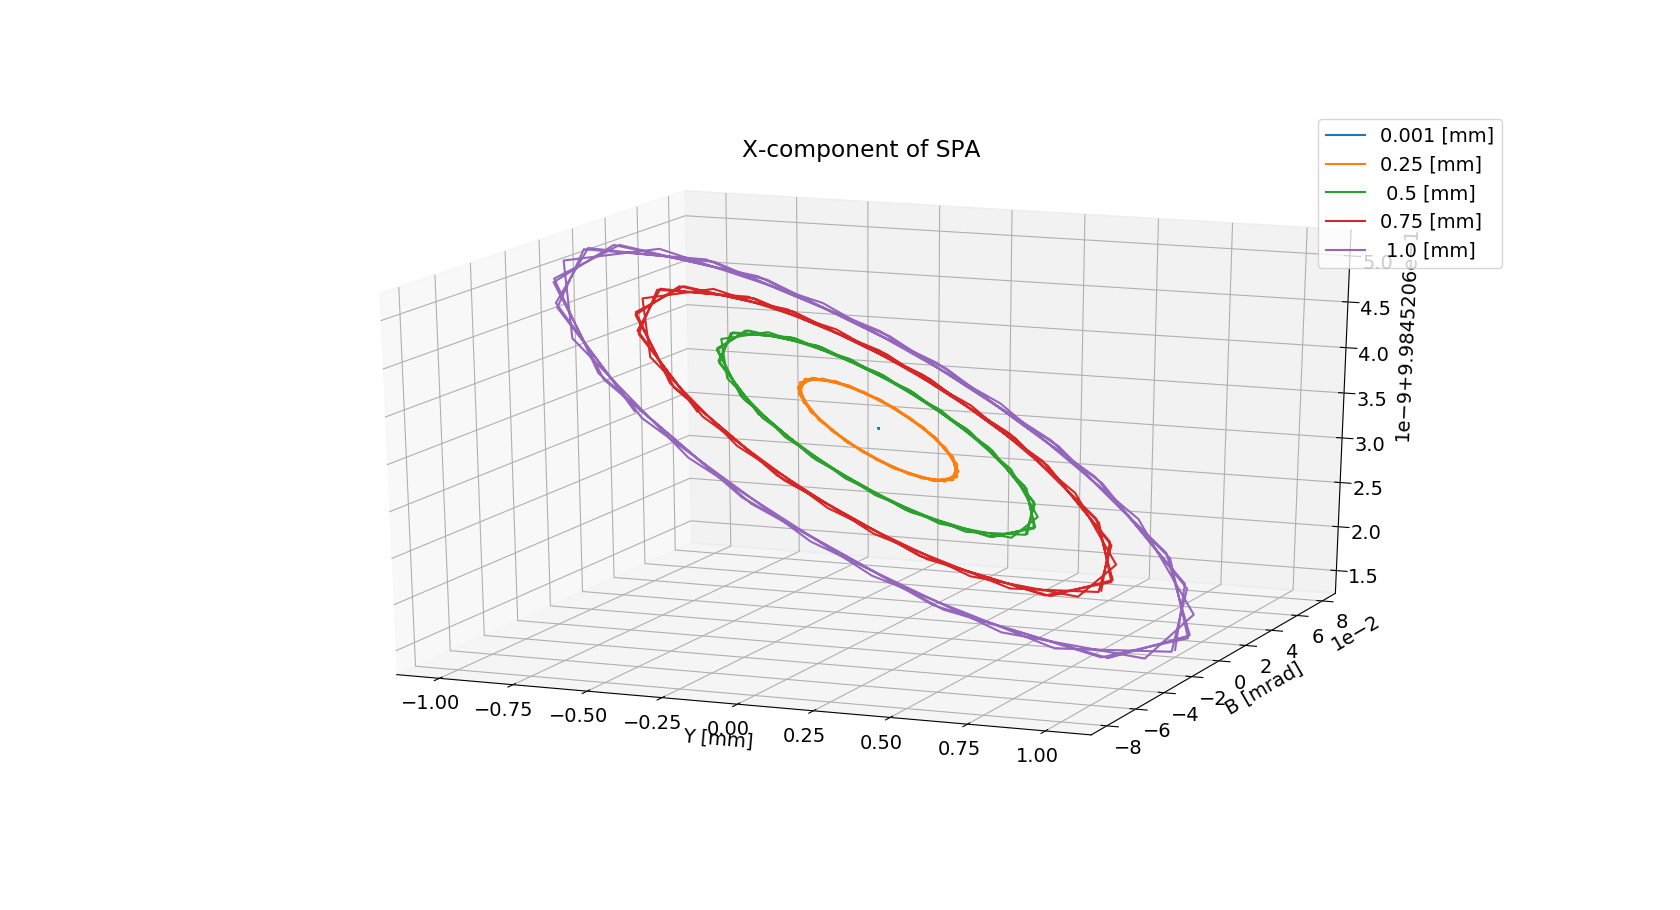
\includegraphics[width=\linewidth]{images/tss_on_betatron/nx}}
	\subbottom[Вертикальная компонента]{%
	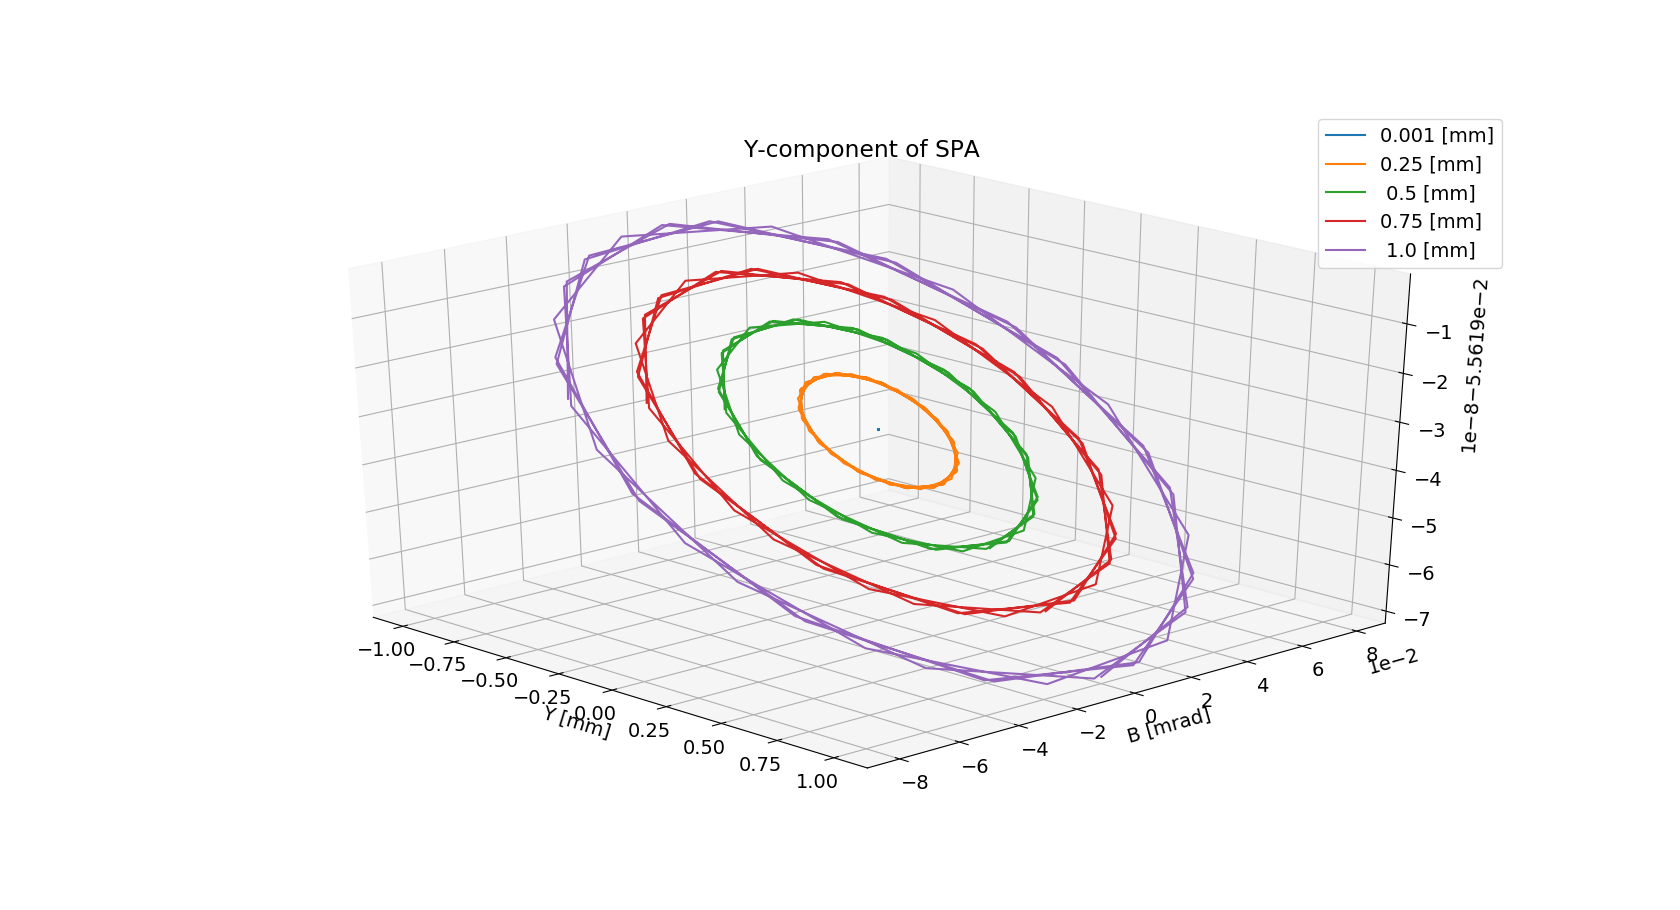
\includegraphics[width=\linewidth]{images/tss_on_betatron/ny}}
\end{figure}
\begin{figure}[h]
	\centering
	\contsubbottom[Продольная компонента]{%
		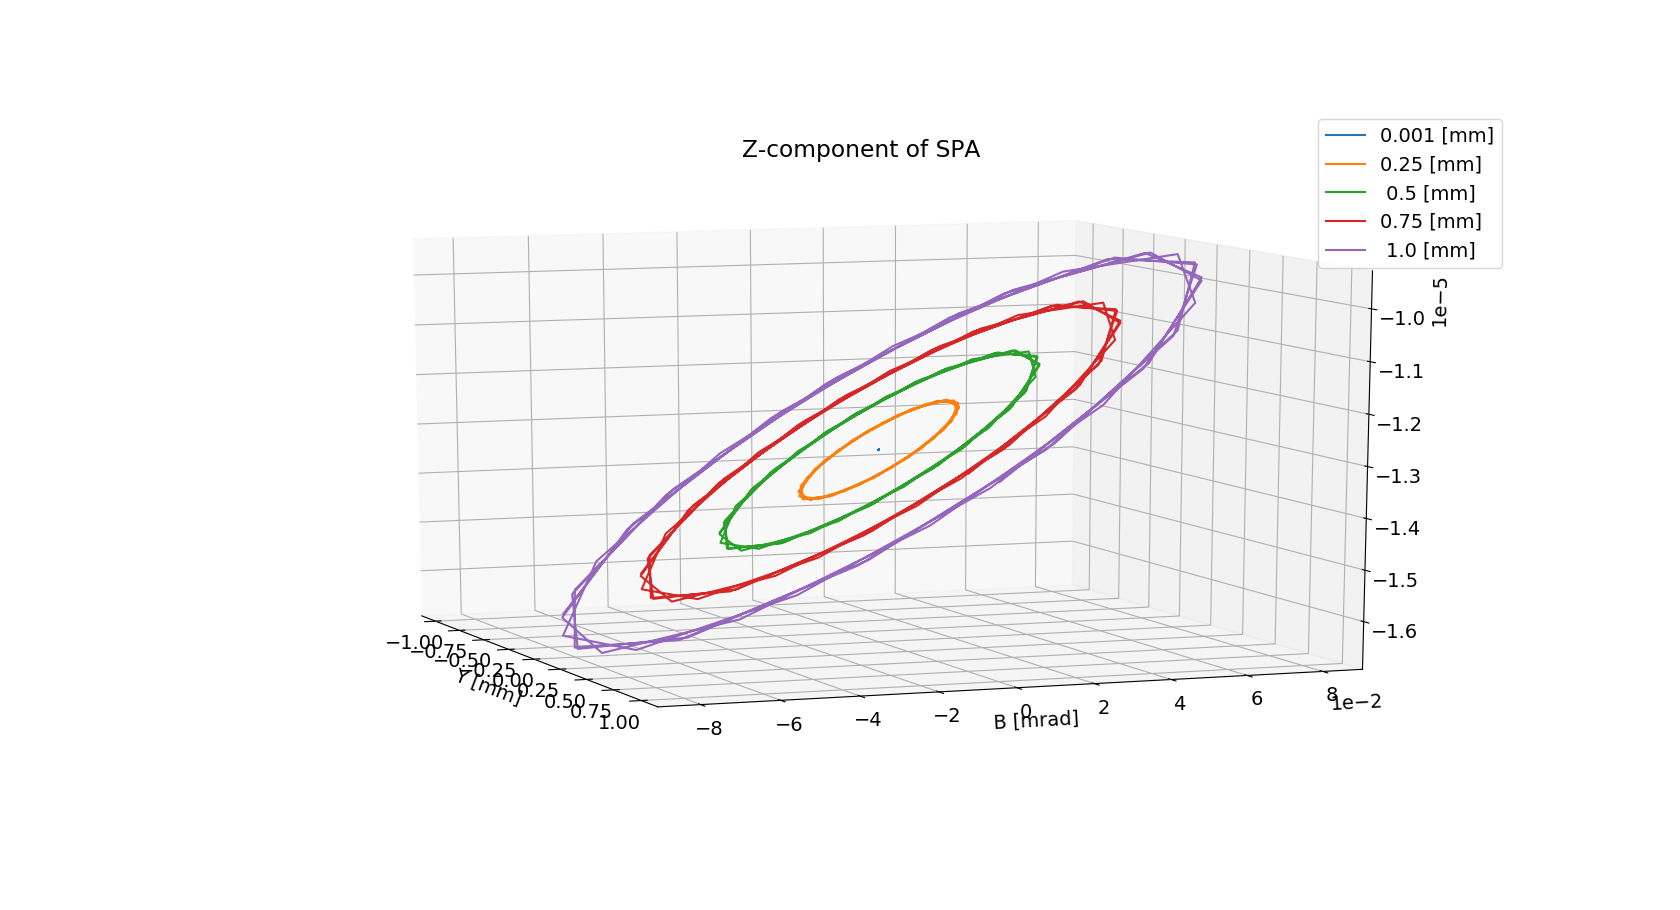
\includegraphics[width=\linewidth]{images/tss_on_betatron/nz}}
	\legend{Цветом обозначены частицы с различным начальным вертикальным смещением от референсной орбиты.}
	\caption{Компоненты оси прецессии спина, вычисленные на фазовых траекториях частиц, после применения секступольных полей для подавления эффекта декогеренции.\label{fig:n-bar_optimized}}
\end{figure}

\begin{figure}[h]
	\centering\hfill
	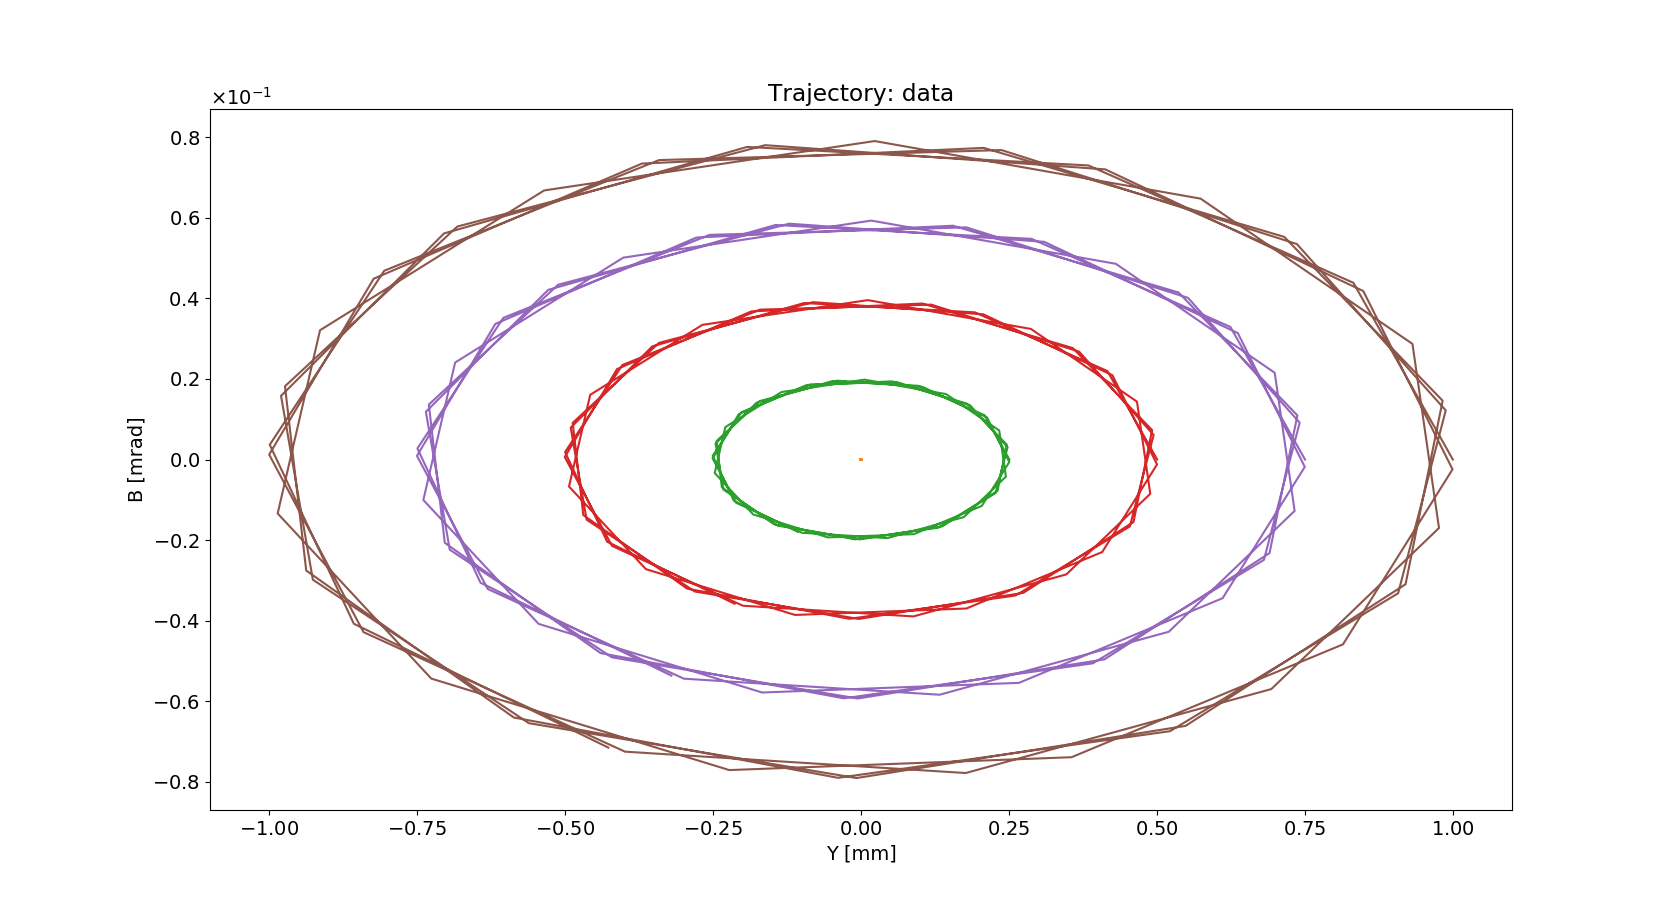
\includegraphics[width=\textwidth]{images/tss_on_betatron/phase_space}
	\caption{Фазовые траектории частиц в ускорителе.\label{fig:phase_space}}
\end{figure}

\begin{figure}[h]
	\centering
	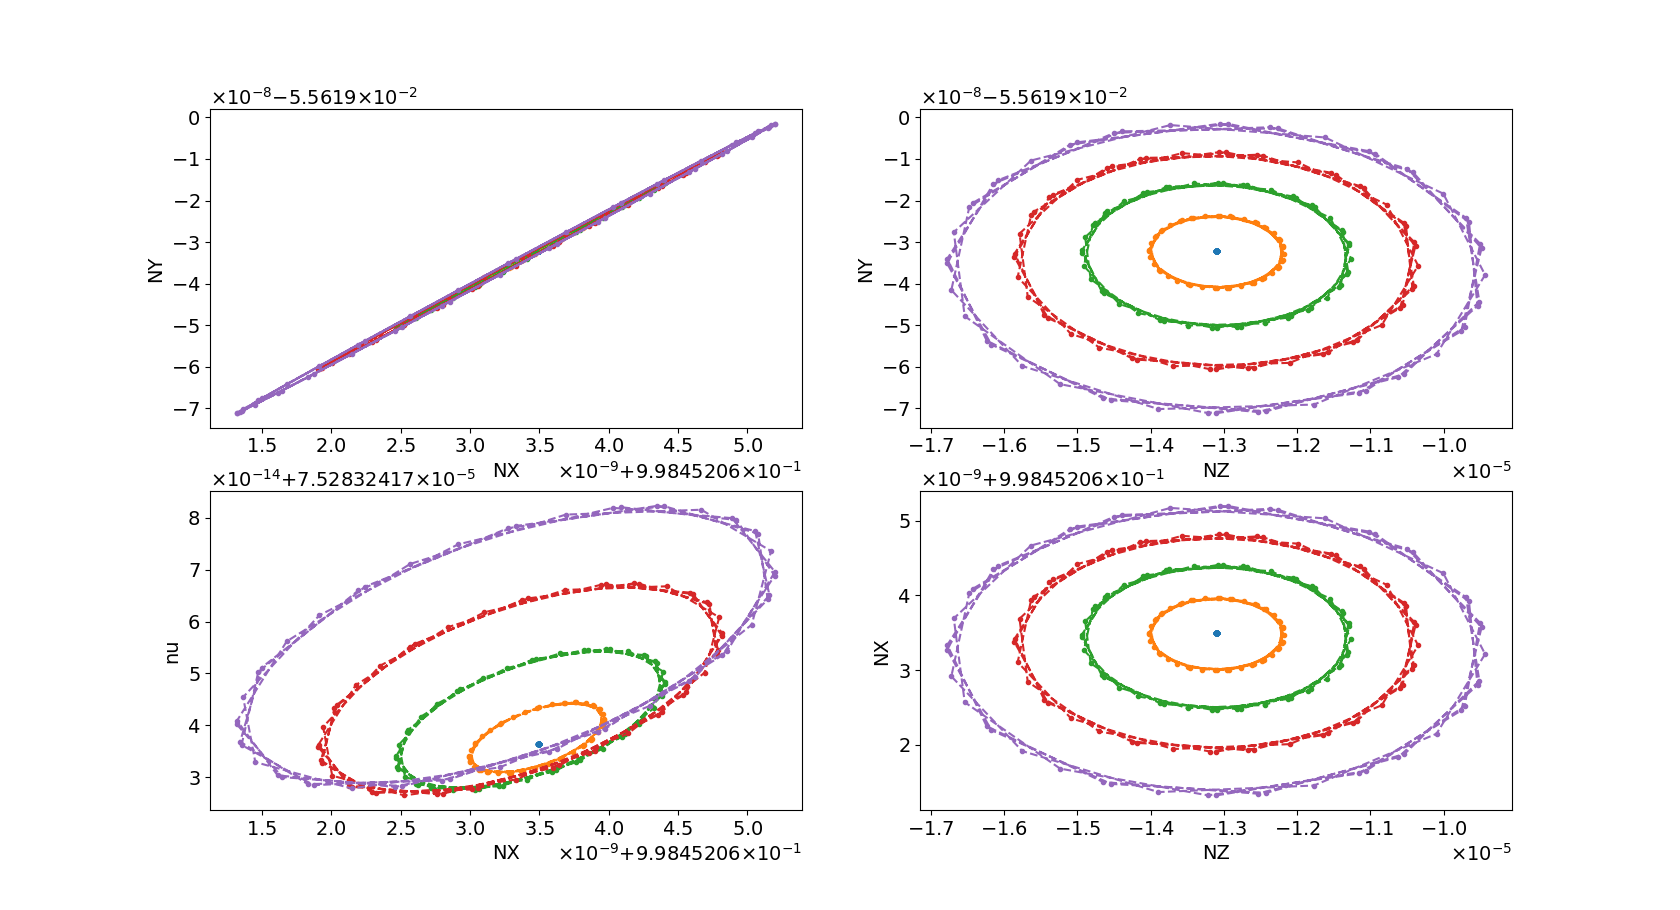
\includegraphics[width=\textwidth]{images/tss_on_betatron/all_vs_all}
	\caption{Компоненты спин-тюна и оси стабильного спина построенные друг против друга.\label{fig:all_vs_all}}
\end{figure}

\subsubsection{Симуляция}
Для подтверждения несущественности эффекта, была проведена следующая симуляция: был выбран ансамбль частиц, смещённых относительно рефернсной орбиты в вертикальном направлении в начальный момент времени. (Начальные значения всех остальных фазовых переменных равны нулю.)

Используя код COSY INFINITY мы протрекали этот ансамбль через структуру с замороженным спином (использующую секступольные поля для подавления декогеренции в вертикальной плоскости) на протяжении 1.2 миллиона оборотов (частота оборота пучка 1 МГц). Каждые 800 оборотов, процедурой TSS~\cite{COSYINF:BeamPhysMan} вычислялись разложения ряда Тейлора третьего порядка для $\nu_s(x,x',y,y',t,\delta)$ и $\bar n(x,x',y,y',t,\delta)$; затем вычислялись значения этих функций в точке фазового пространства, в которой на данный момент находилась частица. Таким образом были получены данные $(\nu_s(t), \bar n(t))$ частиц.

Далее эти данные были использованы для вычисления значений вертикальной компоненты спина $s_y^{func}(t)$ по формуле~\ref{eq:sy_varying_amplitude}. Также в процессе трекинга вычислялись значения $s_y^{data}(t)$ внутренними процедурами COSY INFINITY.

Затем обе серии фитировались функцией $y(t) = a\cdot \sin(2\pi\cdot f\cdot t + \phi)$, в которой оценивались все три параметра $(\hat a,\hat f,\hat \phi)$. Для оптимизации использовался алгоритм Левенберга-Марквардта.

\begin{table}[h]%
	\centering
	\changecaptionwidth\captionwidth{12cm}
	\caption{Результаты фитирования данных\label{tbl:smp-comparison}}
	\begin{tabular}{l|lcl}
		\toprule
		Данные & $\chi^2$ & AIC\footnotemark & $\hat f$, Гц\\
		\midrule
		$s_y^{func}$& $5.4\cdot 10^{-12}$& -49917& $74.452466548 \pm 1\cdot 10^{-9}$\\
		$s_y^{data}$& $2.0\cdot 10^{-6}$& -30665 & $74.452467 \pm 6\cdot 10^{-6}$\\\bottomrule
	\end{tabular}
\end{table}
\footnotetext{Информационный критерий Акаике. Поскольку AIC меньше для данных $s_y^{func}$, можно говорить, что они больше соответствуют синусоидальной модели с постоянной амплитудой и частотой, чем данные, полученные в результате трекинга.}

Исходя из результатов, представленных в Таблице~\ref{tbl:smp-comparison}, можно говорить о том, что прецессия оси стабильного спина не является основной причиной несоответствия данных синусоидальной модели.

\subsection{Декогеренция спинов частиц пучка в идеальном и неидеальном кольцах}
Когеренцией спина называется мера или качество сохранения поляризации
в изначально поляризованном пучке.~\cite[стр.~205]{Eremey:Thesis}

Когда поляризованный пучок инжектируется в накопительное кольцо, спин
векторы частиц пучка начинают прецессировать вокруг вертикального
(ведущего) поля. Частота прецессии зависит от равновесного уровня
энергии частицы, который различен для частиц пучка.

Это обстоятельство не является проблемой в том случае, когда начальная
поляризация пучка вертикальна; однако метод измерения ЭДМ в
накопительном кольце, основанный
на принципе замороженного спина требует, чтобы вектор поляризации
пучка был сонаправлен с его вектором импульса, т.е. лежал в
горизонтальной плоскости. Таким образом, декогеренция спина есть
внутренняя проблема метода замороженного спина.
\subsubsection{Требования ко времени когеренции пучка}
Время когеренции спина (spin coherence time; SCT) для метода
замороженного спина, выполненного в накопительном кольце с идеально
установленными элементами определяется минимальным детектируемым углом
отклонения вектора поляризации пучка из горизонтальной плоскости
только засчёт ЭДМ. Для уровня чувствительности $10^{-29}~e\cdot cm$
это примерно $5\cdot10^{-6}$.~\cite{BNL:Deuteron2008}

В соответствии с уравнением Т-БМТ,
\[
\W_{EDM,x} = \eta\frac{qE_x}{2mc},
\]
где $\eta$ есть коэффициент пропорциональности между ЭДМ и спином,
равный $10^{-15}$ для дейтрона,для данного уровня чувствительности.~\cite[стр.~206]{Eremey:Thesis}

Для дейтронного BNL FS кольца, $E_x = 12$
МВ/м,~\cite[стр.~19]{BNL:Deuteron2008} так что $\W_{EDM,x}\approx
10^{-9}$ рад/сек. Таким образом получаем, что для того, чтобы достичь
детектируемый уровень отклонения вектора поляризации на 1 мкрад требуется SCT порядка 1000 секунд.~\cite[стр.~207]{Eremey:Thesis}
\subsubsection{Происхождение декогеренции}
Декогеренция спина в пучке вызвана разницей угловых скоростей
прецессии спинов частиц, которая, в свою очередь, вызвана разницей
длин орбит и импульсов частиц. Это можно видеть исходя из следующих
соображений.

Когда частица со спином входит в область магнитного поля, её спин-вектор
начинает поворачиваться вокруг вектора магнитного поля с угловой
скоростью определяемой уравнением Т-БМТ~\eqref{eq:TBMT_MDM}:
\begin{equation*}
	\vec\W_{MDM} = \frac qm G\vec B.
\end{equation*}
На выходе из области, вектор спина повёрнут на угол
\begin{equation*}
	\theta = \Delta t\cdot\W_{MDM} = \frac Lv \cdot \frac qm GB\cdot \frac{\gamma_0}{\gamma_0} = \frac{L\gamma_0 GB}{B\rho} = \frac L\rho\gamma_0\cdot G,
\end{equation*}
где $L$ есть длина пути внутри области с магнитным полем, и $B\rho =
p/q$ магнитная жёсткость.

В простой модели рассмотренной выше, влияние орбитальной динамики на
спиновую динамику вырадено через $\gamma_0 L/\rho$ (эффективный
Лоренц-фактор). В случае референсной частицы, $\gamma_0L/\rho =
\gamma_0\alpha$, $\alpha$ угол поворота вектора импульса,в то время
как для частицы участвующей в бетатронном движении, эффективный
Лоренц-фактор больше. В следующих разделах мы выразим связь между
спиновой и орбитальной динамиками частицы в накопительном кольце в
более общих терминах.

\paragraph{Сдвиг равновесного значения импульса частицы.}
Продольная динамика заряженной частицы на референсной орбите в
накопительном кольце описывается системой уравнений
\begin{equation*}
	\begin{cases}
		\ddt{\varphi} &= -\w_{RF}\eta\delta, \\
		\ddt{\delta} &= \frac{q V_{RF}\w_{RF}}{2\pi h\beta^2E}\sin\varphi.
	\end{cases}
\end{equation*}
В уравнениях выше: $\varphi$ отклонение фазы частицы от референсной
$\varphi_0 = 0$; $\delta = \frac{\Delta p}{p_0}$ относительное
отклонение импульса от $p_0$ референсной частицы; $V_{RF}$, $\w_{RF}$
амплитуда и частоты колебаний ВЧ поля; $\eta = \alpha_0 - \gamma^{-2}$
слип-фактор, где $\alpha_0$ --- коэффициент сжатия орбиты, определяемый
через $\sfrac{\Delta L}{L} = \alpha_0\delta$, $L$ длина орбиты; $h$
гармоническое число; $E$ полная энергия ускоряемой частицы. $\w_{RF} =
2\pi h f_{rev}$, где $f_{rev}=T_{rev}^{-1}$ --- частота оборота пучка.

Решения этой системы формируют семейство эллипсов в плоскости
$(\varphi, \delta)$, центрированных на $(0,0)$. Однако, если
рассмотреть частицу, участвующую в бетатронных колебаниях, и
использовать разложение Тейлора более высокого порядка для
коэффициента сжатия орбиты $\alpha = \alpha_0 + \alpha_1\delta$,
первое уравнение системы превратится в:~\cite[стр.~2579]{Senichev:IPAC13}
\[
\ddt{\varphi} = -\w_{RF} \bkt*{\bkt{\frac{\Delta L}{L}}_\beta + \bkt{\alpha_0 + \gamma^{-2}}\delta + \bkt{\alpha_1 - \alpha_0\gamma^{-2} + \gamma^{-4}}\delta^2},
\]
где $\bkt{\frac{\Delta L}{L}}_\beta =
\frac{\pi}{2L}\bkt*{\varepsilon_xQ_x + \varepsilon_yQ_y},$ есть
удлинение орбиты, связанное с бетатронным движением; $\varepsilon_x$ и
$\varepsilon_y$ --- горизонтальный и вертикальный эмиттансы пучка, и
$Q_x$ и $Q_y$ горизонтальный и вертикальный тюны.~\cite[стр.~2580]{Senichev:IPAC13}

Решения модифицированной системы более не центрированы на одной и той
же точке. Удлинение орбиты и отклонение импульса вызывают сдвиг
равновесного значения импульса частицы~\cite[стр.~2581]{Senichev:IPAC13}
\begin{equation}\label{eq:EquLevMom_shift}
\Delta\delta_{eq} = \frac{\gamma_0^2}{\gamma_0^2\alpha_0 - 1}\bkt*{\frac{\delta_m^2}{2}\bkt{\alpha_1 - \alpha_0\gamma^{-2} + \gamma_0^{-4}} + \bkt{\frac{\Delta L}{L}}_\beta},
\end{equation}
где $\delta_m$ --- амплитуда синхротронных колебаний.

\paragraph{Понятие эффективного Лоренц-фактора.}
Равновесное значение энергии, связанное со сдвигом импульса~\eqref{eq:EquLevMom_shift}, и называемое \emph{эффективным Лоренц-фактором}, есть~\cite{Senichev:FDM}
\begin{equation}\label{eq:EffectiveGamma}
\gamma_{eff} = \gamma_0 + \beta_0^2\gamma_0\cdot\Delta\delta_{eq},
\end{equation}
где $\gamma_0$, $\beta_0$ --- Лоренц-фактор референсной частицы и
нормализованное значение
скорости. Уравнения~\eqref{eq:EquLevMom_shift}
и~\eqref{eq:EffectiveGamma} определяют связь между спиновой и
орбитальной динамиками частицы.

Из уравнения для спин-тюна частицы в магнитном поле $\nu_s = \gamma_{eff}\cdot G$ следует, что спин-тюны двух частиц с одинаковыми эффективными Лоренц-факторами равны, независимо от их траекторий в ускорителе. Этот принцип используется при использовании секступольных полей для подавления спиновой декогеренции, а также при смене полярности ведущего магнитного поля кольца.

\subsubsection{Подавление декогеренции с помощью секступольных полей}
Чтобы минимизировать декогеренцию спина, связанную с бетатронным
движением и отклонением импульса, могут быть использованы
секступольные (или октупольные) поля~\cite[стр.~212]{Eremey:Thesis}

Секступоль силы
\[
S_{sext} = \frac{1}{B\rho} \pddx{B_y}[x][2],
\]
где $B\rho$ магнитная жёсткость, влияет на коэффициент сжатия орбиты
первого порядка как~\cite[стр.~2581]{Senichev:IPAC13}
\begin{align}
	\Delta \alpha_{1,sext} &= -\frac{S_{sext}D_0^3}{L}, \label{eq:Sext_compaction_effect}
	\intertext{и одновременно на длину орбиты как}
	\bkt{\frac{\Delta L}{L}}_{sext} &= \mp \frac{S_{sext}D_0\beta_{x,y}\varepsilon_{x,y}}{L}, \label{eq:Sext_OL_effect}
\end{align}
где $D(s,\delta) = D_0(s) + D_1(s)\delta$ обозначает функцию дисперсии.

В следующих разделах мы будем называть декогеренцию, связанную си
горизонтальными/вертикальными бетатронными, и синхротронными
колебаниями соответственно X-/Y-, и D-декогеренцией. 

Из уравнений~\labelcref{eq:Sext_compaction_effect,eq:Sext_OL_effect} можно
видеть, что для подавления декогеренции необходимы три семейства
секступолей, помещённых в максимумы функций: $\beta_x$, $\beta_y$ для подавления
X-,Y-декогеренции, и $D_0$ для D-декогеренции.

\subsection{Фальш-сигнал}\label{sec:systematic_error-fake_signal}
Систематические ошибки, вызванные физическими неидеальностями
ускорителя, включая неточность юстировки оптических элементов,
вызывают фальш-сигнал ЭДМ.~\cite[стр.~230]{Eremey:Thesis} Особенно в
этом отношении проблематичны наклоны элементов вокруг оптической оси, поскльку они
индуцируют паразитные горизонтальные компоненты магнитного поля $B_x$
и $B_z$, которые обе вращают спин в вертикальной плоскости; той, в которой измеряется ЭДМ.

Ю. Сеничевым были сделаны~\cite{Senichev:FDM} аналитические оценки МДМ частоты прецессии спина
вокруг радиальной оси. Из уравнения Т-БМТ, и выражения силы Лоренца,
скорость МДМ прецессии вокруг радиальной оси есть
\begin{equation}
\SD{\W_x^{MDM}} = \frac{q}{m\gamma}\frac{G+1}{\gamma}\frac{\SD{B_x}}{\sqrt{n}},
\end{equation}
где $n$ есть число наклонённых спин-ротаторов, и $\SD{B_x} = B_y
\SD{\delta h}/L$, при стандартном отклонении ошибки юстировки
$\SD{\delta h}$. При величине ошибки $\SD{\delta h} = 100$ мкм, и
длине дефлектора $L=1$ м, $\SD{\W_x^{MDM}} \approx 100$ рад/сек.~\cite{Senichev:FDM}

Мы изучили спиновую динамику в структурах с замороженным и
квази-замороженным спином в присутствии наклонов оптических элементов
с помощью кода COSY INFINITY. Наши симуляции согласуются с оценками,
представленными выше.

\paragraph{Имплементация паразитного поля.}\label{sec:error_field_implementation}
Имплементируя неидеальности полей, мы следовали рекомендациям
изложенным в~\cite[стр.~235]{Eremey:Thesis}. Малое возмущение
магнитного поля, в первом приближении, действует как маленький пропорциональный поворот
спин-вектора. Поэтому мы имплементировали наклон E+B элемента как
домножение соответствующей матрицы поворота на его спиновую матрицу
перехода, ``спин-кик.''

В соответствии с уравнением~\eqref{eq:TBMT_MDM}, изменение МДМ частоты
прецессии, ассоциированное с введённым паразитным полем $(B_x, 0, B_z)$ есть
\begin{align*}
	\Delta\W_{MDM} &= \frac qm (B_x, 0, B_z),
	\intertext{поэтому угол спин-кика равен}
	\Theta_{kick} &= t_0\Delta\W_{MDM},
\end{align*}
где $t_0 = L/v_0$ пролётное время референсной частицы через элемент.
